%--------------------
% Packages
% -------------------
\documentclass[11pt,english]{article}
\usepackage{amsfonts}
\usepackage[left=2.5cm,top=2cm,right=2.5cm,bottom=3cm,bindingoffset=0cm]{geometry}
\usepackage{amsmath, amsthm, amssymb}
\usepackage{tikz}
\usetikzlibrary{calc}
\usetikzlibrary{decorations.pathreplacing,calligraphy}
\usepackage{fancyhdr}
%\usepackage{currfile}
\usepackage{nicefrac}
\usepackage{cite}
\usepackage{graphicx}
\usepackage{caption}
\usepackage{longtable}
\usepackage{rotating}
\usepackage{lscape}
\usepackage{booktabs}
\usepackage{float}
\usepackage{placeins}
\usepackage{setspace}
\usepackage[font=itshape]{quoting}
\onehalfspacing
\usepackage{mathrsfs}
\usepackage{tcolorbox}
\usepackage{xcolor}
\usepackage{subcaption}
\usepackage{float}
\usepackage[multiple]{footmisc}
\usepackage[T1]{fontenc}
\usepackage[sc]{mathpazo}
\usepackage{listings}
\usepackage{longtable}
\definecolor{cmured}{RGB}{175,30,45}
\definecolor{macroblue}{RGB}{56,108,176}
\usepackage[format=plain,
            labelfont=bf,
            textfont=]{caption}
\usepackage[colorlinks=true,citecolor=macroblue,linkcolor=macroblue,urlcolor=macroblue]{hyperref}
\usepackage{varioref}
\usepackage{chngcntr}
\usepackage{datetime}

\definecolor{darkgreen}{RGB}{30,175,88}
\definecolor{darkblue}{RGB}{30,118,175}
\definecolor{maroon}{rgb}{0.66,0,0}
\definecolor{darkgreen}{rgb}{0,0.69,0}

%Counters
\newtheorem{theorem}{Theorem}[section] 
\newtheorem{proposition}{Proposition}
\newtheorem{lemma}{Lemma}
\newtheorem{corollary}{Corollary}
\newtheorem{assumption}{Assumption}
\newtheorem{axiom}{Axiom}
\newtheorem{case}{Case}
\newtheorem{claim}{Claim}
\newtheorem{condition}{Condition}
\newtheorem{definition}{Definition}
\newtheorem{example}{Example}
\newtheorem{notation}{Notation}
\newtheorem{remark}{Remark}


\hypersetup{ 	
pdfsubject = {},
pdftitle = {TidyTuesday Week 42},
pdfauthor = {Pranay Gundam},
linkcolor= macroblue
}


\title{\textbf{TidyTuesday Week 42}}
\author{Pranay Gundam}


%-----------------------
% Begin document
%-----------------------
\begin{document}

\maketitle

\tableofcontents

\section{Weekly Summary}


\section{Date: 2024-10-15}
\noindent \textbf{Series ID: MORTGAGE15W} 

\noindent This series is titled 15-Year Fixed Rate Mortgage Average in the West Freddie Mac Region (DISCONTINUED) and has a frequency of Weekly, Ending Thursday. The units are Percent and the seasonal adjustment is Not Seasonally Adjusted.The observation start date is 1991-08-30 and the observation end date is 2015-12-31.The popularity of this series is 1. \\ 

\noindent \textbf{Series ID: RTWVDMI684NMFRBDAL} 

\noindent This series is titled Real Trade-Weighted Value of the dollar for Michigan (DISCONTINUED) and has a frequency of Monthly. The units are Index Jan 1988=100 and the seasonal adjustment is Not Seasonally Adjusted.The observation start date is 1988-01-01 and the observation end date is 2023-06-01.The popularity of this series is 1. \\ 

\subsection{Regression Tables and Plots}
\begin{center}
\begin{tabular}{lclc}
\toprule
\textbf{Dep. Variable:}           & value\_fred\_RTWVDMI684NMFRBDAL & \textbf{  R-squared:         } &     0.195   \\
\textbf{Model:}                   &               OLS               & \textbf{  Adj. R-squared:    } &     0.173   \\
\textbf{Method:}                  &          Least Squares          & \textbf{  F-statistic:       } &     8.725   \\
\textbf{Date:}                    &         Tue, 15 Oct 2024        & \textbf{  Prob (F-statistic):} &  0.00550    \\
\textbf{Time:}                    &             18:54:33            & \textbf{  Log-Likelihood:    } &   -141.53   \\
\textbf{No. Observations:}        &                  38             & \textbf{  AIC:               } &     287.1   \\
\textbf{Df Residuals:}            &                  36             & \textbf{  BIC:               } &     290.3   \\
\textbf{Df Model:}                &                   1             & \textbf{                     } &             \\
\textbf{Covariance Type:}         &            nonrobust            & \textbf{                     } &             \\
\bottomrule
\end{tabular}
\begin{tabular}{lcccccc}
                                  & \textbf{coef} & \textbf{std err} & \textbf{t} & \textbf{P$> |$t$|$} & \textbf{[0.025} & \textbf{0.975]}  \\
\midrule
\textbf{const}                    &      84.9099  &        6.171     &    13.760  &         0.000        &       72.395    &       97.425     \\
\textbf{value\_fred\_MORTGAGE15W} &       3.0350  &        1.027     &     2.954  &         0.006        &        0.951    &        5.119     \\
\bottomrule
\end{tabular}
\begin{tabular}{lclc}
\textbf{Omnibus:}       &  0.436 & \textbf{  Durbin-Watson:     } &    0.277  \\
\textbf{Prob(Omnibus):} &  0.804 & \textbf{  Jarque-Bera (JB):  } &    0.449  \\
\textbf{Skew:}          &  0.231 & \textbf{  Prob(JB):          } &    0.799  \\
\textbf{Kurtosis:}      &  2.735 & \textbf{  Cond. No.          } &     22.7  \\
\bottomrule
\end{tabular}
%\caption{OLS Regression Results}
\end{center}

Notes: \newline
 [1] Standard Errors assume that the covariance matrix of the errors is correctly specified.

\begin{figure}
\centering
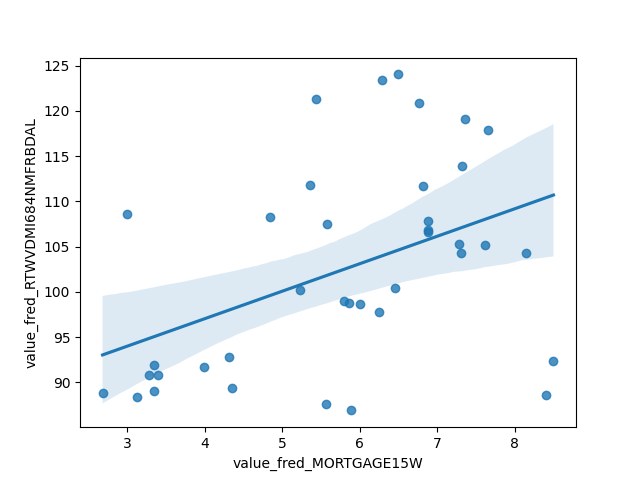
\includegraphics[scale = 0.9]{plots/plot_2024-10-15.png}
\caption{Regression Plot for 2024-10-15}
\end{figure}
\newpage

\section{Date: 2024-10-16}
\noindent \textbf{Series ID: ATNHPIUS33140Q} 

\noindent This series is titled All-Transactions House Price Index for Michigan City-La Porte, IN (MSA) and has a frequency of Quarterly. The units are Index 1995:Q1=100 and the seasonal adjustment is Not Seasonally Adjusted.The observation start date is 1986-04-01 and the observation end date is 2024-04-01.The popularity of this series is 1. \\ 

\noindent \textbf{Series ID: DRALT100S} 

\noindent This series is titled Delinquency Rate on All Loans, Banks Ranked 1st to 100th Largest in Size by Assets and has a frequency of Quarterly, End of Period. The units are Percent and the seasonal adjustment is Seasonally Adjusted.The observation start date is 1985-01-01 and the observation end date is 2024-04-01.The popularity of this series is 26. \\ 

\subsection{Regression Tables and Plots}
\begin{center}
\begin{tabular}{lclc}
\toprule
\textbf{Dep. Variable:}              & value\_fred\_DRALT100S & \textbf{  R-squared:         } &     0.310   \\
\textbf{Model:}                      &          OLS           & \textbf{  Adj. R-squared:    } &     0.305   \\
\textbf{Method:}                     &     Least Squares      & \textbf{  F-statistic:       } &     67.73   \\
\textbf{Date:}                       &    Wed, 16 Oct 2024    & \textbf{  Prob (F-statistic):} &  8.12e-14   \\
\textbf{Time:}                       &        09:58:41        & \textbf{  Log-Likelihood:    } &   -289.22   \\
\textbf{No. Observations:}           &            153         & \textbf{  AIC:               } &     582.4   \\
\textbf{Df Residuals:}               &            151         & \textbf{  BIC:               } &     588.5   \\
\textbf{Df Model:}                   &              1         & \textbf{                     } &             \\
\textbf{Covariance Type:}            &       nonrobust        & \textbf{                     } &             \\
\bottomrule
\end{tabular}
\begin{tabular}{lcccccc}
                                     & \textbf{coef} & \textbf{std err} & \textbf{t} & \textbf{P$> |$t$|$} & \textbf{[0.025} & \textbf{0.975]}  \\
\midrule
\textbf{const}                       &       6.3015  &        0.376     &    16.750  &         0.000        &        5.558    &        7.045     \\
\textbf{value\_fred\_ATNHPIUS33140Q} &      -0.0204  &        0.002     &    -8.230  &         0.000        &       -0.025    &       -0.015     \\
\bottomrule
\end{tabular}
\begin{tabular}{lclc}
\textbf{Omnibus:}       & 22.326 & \textbf{  Durbin-Watson:     } &    0.035  \\
\textbf{Prob(Omnibus):} &  0.000 & \textbf{  Jarque-Bera (JB):  } &   27.308  \\
\textbf{Skew:}          &  1.012 & \textbf{  Prob(JB):          } & 1.18e-06  \\
\textbf{Kurtosis:}      &  3.431 & \textbf{  Cond. No.          } &     439.  \\
\bottomrule
\end{tabular}
%\caption{OLS Regression Results}
\end{center}

Notes: \newline
 [1] Standard Errors assume that the covariance matrix of the errors is correctly specified.

\begin{figure}
\centering
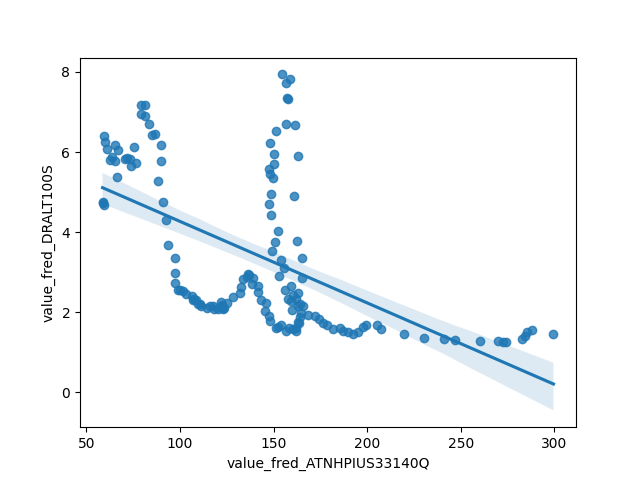
\includegraphics[scale = 0.9]{plots/plot_2024-10-16.png}
\caption{Regression Plot for 2024-10-16}
\end{figure}
\newpage

\section{Date: 2024-10-17}
\noindent \textbf{Series ID: EXP0017} 

\noindent This series is titled U.S. Exports of Goods by F.A.S. Basis to CAFTA-DR and has a frequency of Monthly. The units are Millions of Dollars and the seasonal adjustment is Not Seasonally Adjusted.The observation start date is 2005-01-01 and the observation end date is 2024-08-01.The popularity of this series is 1. \\ 

\noindent \textbf{Series ID: IY111} 

\noindent This series is titled Export Price Index (NAICS): Crop Production and has a frequency of Monthly. The units are Index Dec 2005=100 and the seasonal adjustment is Not Seasonally Adjusted.The observation start date is 2005-12-01 and the observation end date is 2024-09-01.The popularity of this series is 3. \\ 

\subsection{Regression Tables and Plots}
\begin{center}
\begin{tabular}{lclc}
\toprule
\textbf{Dep. Variable:}       & value\_fred\_IY111 & \textbf{  R-squared:         } &     0.518   \\
\textbf{Model:}               &        OLS         & \textbf{  Adj. R-squared:    } &     0.516   \\
\textbf{Method:}              &   Least Squares    & \textbf{  F-statistic:       } &     239.5   \\
\textbf{Date:}                &  Thu, 17 Oct 2024  & \textbf{  Prob (F-statistic):} &  3.52e-37   \\
\textbf{Time:}                &      08:35:17      & \textbf{  Log-Likelihood:    } &   -1045.4   \\
\textbf{No. Observations:}    &          225       & \textbf{  AIC:               } &     2095.   \\
\textbf{Df Residuals:}        &          223       & \textbf{  BIC:               } &     2102.   \\
\textbf{Df Model:}            &            1       & \textbf{                     } &             \\
\textbf{Covariance Type:}     &     nonrobust      & \textbf{                     } &             \\
\bottomrule
\end{tabular}
\begin{tabular}{lcccccc}
                              & \textbf{coef} & \textbf{std err} & \textbf{t} & \textbf{P$> |$t$|$} & \textbf{[0.025} & \textbf{0.975]}  \\
\midrule
\textbf{const}                &      80.7007  &        6.464     &    12.485  &         0.000        &       67.963    &       93.438     \\
\textbf{value\_fred\_EXP0017} &       0.0376  &        0.002     &    15.475  &         0.000        &        0.033    &        0.042     \\
\bottomrule
\end{tabular}
\begin{tabular}{lclc}
\textbf{Omnibus:}       &  9.298 & \textbf{  Durbin-Watson:     } &    0.195  \\
\textbf{Prob(Omnibus):} &  0.010 & \textbf{  Jarque-Bera (JB):  } &    8.903  \\
\textbf{Skew:}          &  0.436 & \textbf{  Prob(JB):          } &   0.0117  \\
\textbf{Kurtosis:}      &  2.565 & \textbf{  Cond. No.          } & 1.02e+04  \\
\bottomrule
\end{tabular}
%\caption{OLS Regression Results}
\end{center}

Notes: \newline
 [1] Standard Errors assume that the covariance matrix of the errors is correctly specified. \newline
 [2] The condition number is large, 1.02e+04. This might indicate that there are \newline
 strong multicollinearity or other numerical problems.

\begin{figure}
\centering
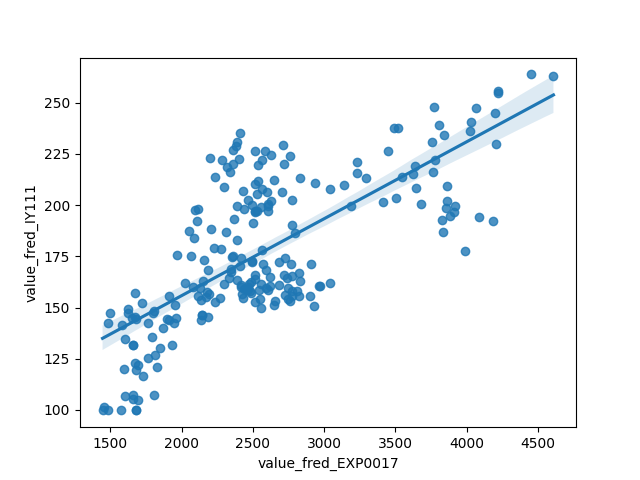
\includegraphics[scale = 0.9]{plots/plot_2024-10-17.png}
\caption{Regression Plot for 2024-10-17}
\end{figure}
\newpage

\section{Date: 2024-10-18}
\noindent \textbf{Series ID: BRVSLV02JPQ460S} 

\noindent This series is titled Business Tendency Surveys: Volume of Stocks: Economic Activity: Retail Trade, Except of Motor Vehicles and Motorcycles: Current for Japan and has a frequency of Quarterly. The units are Percentage balance and the seasonal adjustment is Seasonally Adjusted.The observation start date is 1990-10-01 and the observation end date is 2024-04-01.The popularity of this series is 1. \\ 

\noindent \textbf{Series ID: CIU2016000000000I} 

\noindent This series is titled Employment Cost Index: Total compensation for Private industry workers in Education and health services and has a frequency of Quarterly. The units are Index Dec 2005=100 and the seasonal adjustment is Not Seasonally Adjusted.The observation start date is 2001-01-01 and the observation end date is 2024-04-01.The popularity of this series is 0. \\ 

\subsection{Regression Tables and Plots}
\begin{center}
\begin{tabular}{lclc}
\toprule
\textbf{Dep. Variable:}               & value\_fred\_CIU2016000000000I & \textbf{  R-squared:         } &     0.491   \\
\textbf{Model:}                       &              OLS               & \textbf{  Adj. R-squared:    } &     0.485   \\
\textbf{Method:}                      &         Least Squares          & \textbf{  F-statistic:       } &     88.72   \\
\textbf{Date:}                        &        Fri, 18 Oct 2024        & \textbf{  Prob (F-statistic):} &  3.81e-15   \\
\textbf{Time:}                        &            10:29:03            & \textbf{  Log-Likelihood:    } &   -384.76   \\
\textbf{No. Observations:}            &                 94             & \textbf{  AIC:               } &     773.5   \\
\textbf{Df Residuals:}                &                 92             & \textbf{  BIC:               } &     778.6   \\
\textbf{Df Model:}                    &                  1             & \textbf{                     } &             \\
\textbf{Covariance Type:}             &           nonrobust            & \textbf{                     } &             \\
\bottomrule
\end{tabular}
\begin{tabular}{lcccccc}
                                      & \textbf{coef} & \textbf{std err} & \textbf{t} & \textbf{P$> |$t$|$} & \textbf{[0.025} & \textbf{0.975]}  \\
\midrule
\textbf{const}                        &     138.6274  &        2.544     &    54.495  &         0.000        &      133.575    &      143.680     \\
\textbf{value\_fred\_BRVSLV02JPQ460S} &      -1.7169  &        0.182     &    -9.419  &         0.000        &       -2.079    &       -1.355     \\
\bottomrule
\end{tabular}
\begin{tabular}{lclc}
\textbf{Omnibus:}       &  2.430 & \textbf{  Durbin-Watson:     } &    0.195  \\
\textbf{Prob(Omnibus):} &  0.297 & \textbf{  Jarque-Bera (JB):  } &    1.900  \\
\textbf{Skew:}          & -0.191 & \textbf{  Prob(JB):          } &    0.387  \\
\textbf{Kurtosis:}      &  2.418 & \textbf{  Cond. No.          } &     23.6  \\
\bottomrule
\end{tabular}
%\caption{OLS Regression Results}
\end{center}

Notes: \newline
 [1] Standard Errors assume that the covariance matrix of the errors is correctly specified.

\begin{figure}
\centering
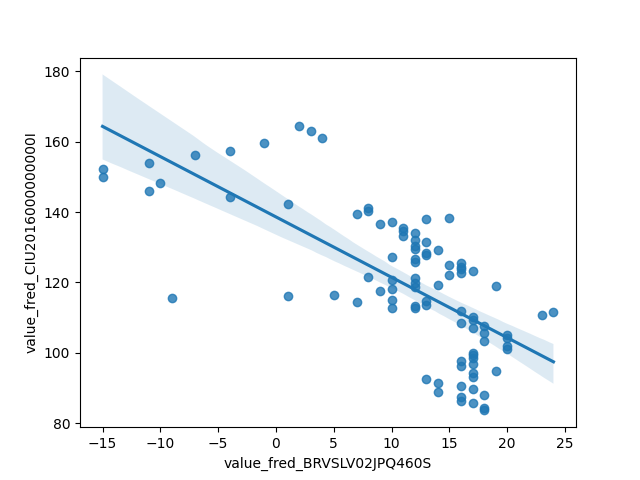
\includegraphics[scale = 0.9]{plots/plot_2024-10-18.png}
\caption{Regression Plot for 2024-10-18}
\end{figure}
\newpage

\section{Date: 2024-10-19}
\noindent \textbf{Series ID: CSHICPROA156NRUG} 

\noindent This series is titled Share of Gross Capital Formation at Current Purchasing Power Parities for Romania and has a frequency of Annual. The units are Percent and the seasonal adjustment is Not Seasonally Adjusted.The observation start date is 1960-01-01 and the observation end date is 2019-01-01.The popularity of this series is 0. \\ 

\noindent \textbf{Series ID: BEAGLBPPRIV} 

\noindent This series is titled New Private Housing Units Authorized by Building Permit for the Great Lakes BEA Region and has a frequency of Monthly. The units are Units and the seasonal adjustment is Not Seasonally Adjusted.The observation start date is 1988-01-01 and the observation end date is 2017-06-01.The popularity of this series is 1. \\ 

\subsection{Regression Tables and Plots}
\begin{center}
\begin{tabular}{lclc}
\toprule
\textbf{Dep. Variable:}                & value\_fred\_BEAGLBPPRIV & \textbf{  R-squared:         } &     0.321   \\
\textbf{Model:}                        &           OLS            & \textbf{  Adj. R-squared:    } &     0.297   \\
\textbf{Method:}                       &      Least Squares       & \textbf{  F-statistic:       } &     13.25   \\
\textbf{Date:}                         &     Sat, 19 Oct 2024     & \textbf{  Prob (F-statistic):} &  0.00109    \\
\textbf{Time:}                         &         10:17:59         & \textbf{  Log-Likelihood:    } &   -281.13   \\
\textbf{No. Observations:}             &              30          & \textbf{  AIC:               } &     566.3   \\
\textbf{Df Residuals:}                 &              28          & \textbf{  BIC:               } &     569.1   \\
\textbf{Df Model:}                     &               1          & \textbf{                     } &             \\
\textbf{Covariance Type:}              &        nonrobust         & \textbf{                     } &             \\
\bottomrule
\end{tabular}
\begin{tabular}{lcccccc}
                                       & \textbf{coef} & \textbf{std err} & \textbf{t} & \textbf{P$> |$t$|$} & \textbf{[0.025} & \textbf{0.975]}  \\
\midrule
\textbf{const}                         &    1.504e+04  &     1986.264     &     7.574  &         0.000        &      1.1e+04    &     1.91e+04     \\
\textbf{value\_fred\_CSHICPROA156NRUG} &   -3.503e+04  &     9624.625     &    -3.640  &         0.001        &    -5.47e+04    &    -1.53e+04     \\
\bottomrule
\end{tabular}
\begin{tabular}{lclc}
\textbf{Omnibus:}       &  4.278 & \textbf{  Durbin-Watson:     } &    0.829  \\
\textbf{Prob(Omnibus):} &  0.118 & \textbf{  Jarque-Bera (JB):  } &    3.730  \\
\textbf{Skew:}          &  0.855 & \textbf{  Prob(JB):          } &    0.155  \\
\textbf{Kurtosis:}      &  2.751 & \textbf{  Cond. No.          } &     18.6  \\
\bottomrule
\end{tabular}
%\caption{OLS Regression Results}
\end{center}

Notes: \newline
 [1] Standard Errors assume that the covariance matrix of the errors is correctly specified.

\begin{figure}
\centering
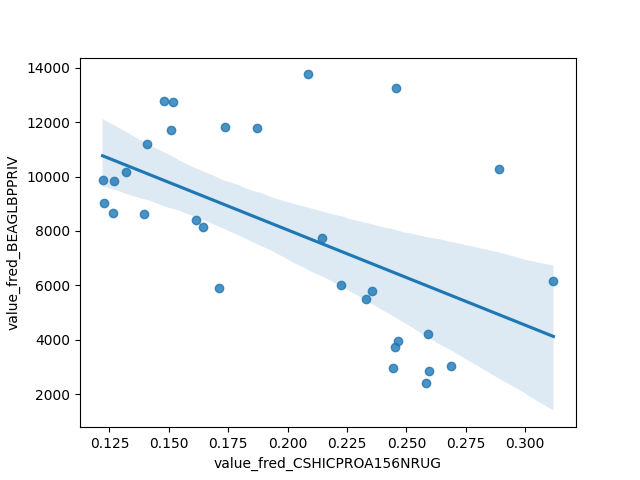
\includegraphics[scale = 0.9]{plots/plot_2024-10-19.png}
\caption{Regression Plot for 2024-10-19}
\end{figure}
\newpage

\include{tex_things/day_2024-10-20}
\section{Date: 2024-10-21}
\noindent \textbf{Series ID: CGDPESMZA666NRUG} 

\noindent This series is titled Expenditure-side Real GDP at Current Purchasing Power Parities for Mozambique and has a frequency of Annual. The units are Millions of 2017 U.S. Dollars and the seasonal adjustment is Not Seasonally Adjusted.The observation start date is 1960-01-01 and the observation end date is 2019-01-01.The popularity of this series is 1. \\ 

\noindent \textbf{Series ID: IR14200} 

\noindent This series is titled Import Price Index (End Use): Bauxite and Aluminum and has a frequency of Monthly. The units are Index 2000=100 and the seasonal adjustment is Not Seasonally Adjusted.The observation start date is 1986-09-01 and the observation end date is 2024-09-01.The popularity of this series is 38. \\ 

\subsection{Regression Tables and Plots}
\begin{center}
\begin{tabular}{lclc}
\toprule
\textbf{Dep. Variable:}                & value\_fred\_IR14200 & \textbf{  R-squared:         } &     0.588   \\
\textbf{Model:}                        &         OLS          & \textbf{  Adj. R-squared:    } &     0.571   \\
\textbf{Method:}                       &    Least Squares     & \textbf{  F-statistic:       } &     34.30   \\
\textbf{Date:}                         &   Mon, 21 Oct 2024   & \textbf{  Prob (F-statistic):} &  4.85e-06   \\
\textbf{Time:}                         &       13:41:09       & \textbf{  Log-Likelihood:    } &   -109.92   \\
\textbf{No. Observations:}             &            26        & \textbf{  AIC:               } &     223.8   \\
\textbf{Df Residuals:}                 &            24        & \textbf{  BIC:               } &     226.3   \\
\textbf{Df Model:}                     &             1        & \textbf{                     } &             \\
\textbf{Covariance Type:}              &      nonrobust       & \textbf{                     } &             \\
\bottomrule
\end{tabular}
\begin{tabular}{lcccccc}
                                       & \textbf{coef} & \textbf{std err} & \textbf{t} & \textbf{P$> |$t$|$} & \textbf{[0.025} & \textbf{0.975]}  \\
\midrule
\textbf{const}                         &      66.0597  &        9.716     &     6.799  &         0.000        &       46.006    &       86.113     \\
\textbf{value\_fred\_CGDPESMZA666NRUG} &       0.0023  &        0.000     &     5.857  &         0.000        &        0.002    &        0.003     \\
\bottomrule
\end{tabular}
\begin{tabular}{lclc}
\textbf{Omnibus:}       &  0.668 & \textbf{  Durbin-Watson:     } &    1.165  \\
\textbf{Prob(Omnibus):} &  0.716 & \textbf{  Jarque-Bera (JB):  } &    0.640  \\
\textbf{Skew:}          &  0.334 & \textbf{  Prob(JB):          } &    0.726  \\
\textbf{Kurtosis:}      &  2.620 & \textbf{  Cond. No.          } & 7.00e+04  \\
\bottomrule
\end{tabular}
%\caption{OLS Regression Results}
\end{center}

Notes: \newline
 [1] Standard Errors assume that the covariance matrix of the errors is correctly specified. \newline
 [2] The condition number is large,  7e+04. This might indicate that there are \newline
 strong multicollinearity or other numerical problems.

\begin{figure}
\centering
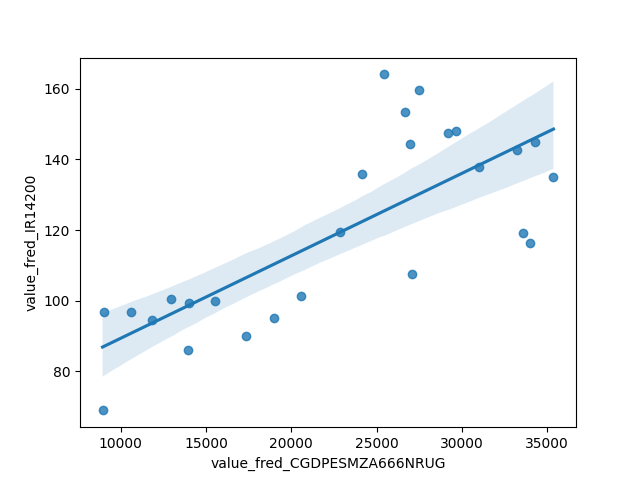
\includegraphics[scale = 0.9]{plots/plot_2024-10-21.png}
\caption{Regression Plot for 2024-10-21}
\end{figure}
\newpage


\end{document}
